\documentclass{article}
\usepackage[utf8]{inputenc}

\title{Assignment-4\\Fork assignment-3}
\author{Subash Mylraj \\(CED18I051) }
\date{16 September 2020}

\usepackage{geometry}
 \geometry{
 a4paper,
 total={170mm,257mm},
 left=20mm,
 top=10mm,
 }

\usepackage{longtable}
\usepackage{graphicx}
\usepackage{listings}
\usepackage{xcolor}

\begin{document}

\maketitle

\lstset{
  language=c,
  aboveskip=3mm,
  belowskip=3mm,
  showstringspaces=false,
  columns=flexible,
  basicstyle={\small\ttfamily},
  numbers=none,
  numberstyle=\tiny\color{gray},
  keywordstyle=\color{blue},
  commentstyle=\color{dkgreen},
  stringstyle=\color{mauve},
  breaklines=true,
  breakatwhitespace=true,
  tabsize=3
}

\definecolor{dkgreen}{rgb}{0,0.6,0}
\definecolor{gray}{rgb}{0.5,0.5,0.5}
\definecolor{mauve}{rgb}{0.58,0,0.82}

\section*{Question 1: Test drive a C program that creates Orphan and Zombie Processes.}
\bigskip

\textbf{\Large Code: Zombie}
\smallskip
\par\noindent\rule{\textwidth}{0.4pt}
\lstinputlisting[language=c]{src/1_zombie.c}
\par\noindent\rule{\textwidth}{0.4pt}

\bigskip
\noindent
\textbf{\Large Output:}

\begin{figure}[h]
	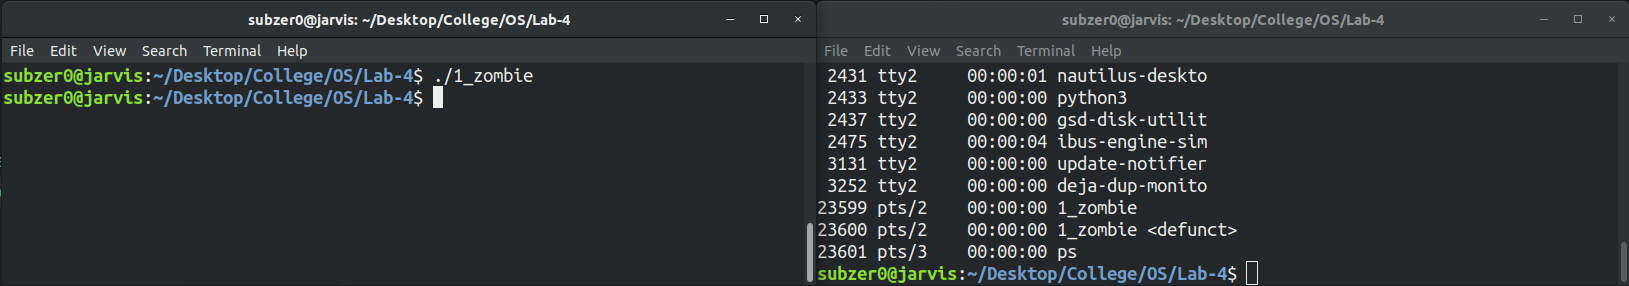
\includegraphics[width=\textwidth]{output/1_zombie.png}
\end{figure}

\bigskip
\bigskip
\par\noindent
\textbf{\Large Code: Orphan}
\smallskip
\par\noindent\rule{\textwidth}{0.4pt}
\lstinputlisting[language=c]{src/1_orphan.c}
\par\noindent\rule{\textwidth}{0.4pt}

\bigskip
\noindent
\textbf{\Large Output:}

\begin{figure}[h]
	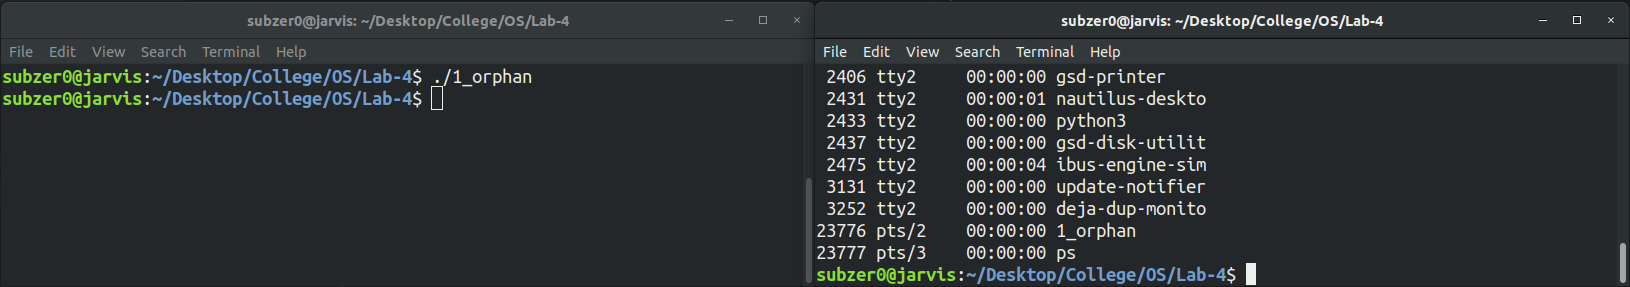
\includegraphics[width=\textwidth]{output/1_orphan.png}
\end{figure}
\bigskip


\section*{Question 2: Develop a multiprocessing version of Merge or Quick Sort. Extra credits would be given for those who implement both in a multiprocessing fashion [ increased no of processes to enhance the effect of parallelization]}
\bigskip

\textbf{\Large Code:}
\smallskip
\par\noindent\rule{\textwidth}{0.4pt}
\lstinputlisting[language=c]{src/2.c}
\par\noindent\rule{\textwidth}{0.4pt}

\bigskip
\noindent
\textbf{\Large Explanation: } \\

The above code is a multiprocessing implementation of merge sort. Basically,
every division is done by a new process. Every merge is done by a process 
when its subproblems are completed. Hence, the placement of waitpid() can be justified.
\\Shared memory was used to make sure that the changes done to the array are available across
all the processes.

\bigskip
\noindent
\textbf{\Large Output:}

\begin{figure}[h]
	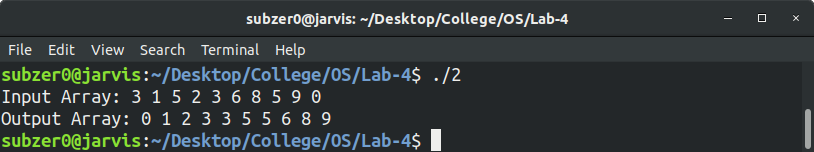
\includegraphics[width=\textwidth]{output/2.png}
\end{figure}
\bigskip


\section*{Question 3: Develop a C program to count the maximum number of processes that can be created using fork call.}
\bigskip

\textbf{\Large Code:}
\smallskip
\par\noindent\rule{\textwidth}{0.4pt}
\lstinputlisting[language=c]{src/3.c}
\par\noindent\rule{\textwidth}{0.4pt}

\bigskip
\noindent
\textbf{\Large Explanation: } \\

	This code creates child processes in an infinite loop till 
	it reaches a point when it cannot create anymore processes.
	This limit can be assumed as the cap on the number of processes
	that can be created. \\

	To avoid the issue of child processes calling fork repeatedly,
	the child processes are made to sleep for a time of 10 seconds.
	So essentially, this program finds the total number of processes
	that can be created in about 10 seconds (its a bit more than 10
	seconds as there is time taken for context switching and other 
	statements). Increasing the sleep time for each process, produced
	similar results.

\bigskip
\noindent
\textbf{\Large Output:}

\begin{figure}[h]
	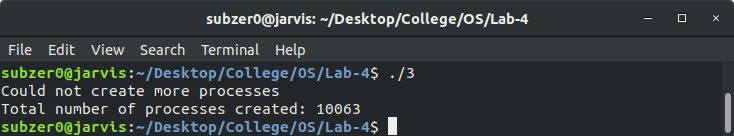
\includegraphics[width=\textwidth]{output/3.png}
\end{figure}
\bigskip

\section*{Question 4: Develop your own command shell [say mark it with @] that accepts user commands (System or User Binaries), executes the commands and returns the prompt for further user interaction. Also extend this to support a history feature (if the user types !6 at the command prompt; it shud display the most recent execute 6 commands). You may provide validation features such as !10 when there are only 9 files to display the entire history contents and other validations required for the history feature;}
\bigskip

\textbf{\Large Code:}
\smallskip
\par\noindent\rule{\textwidth}{0.4pt}
\lstinputlisting[language=c]{src/4.c}
\par\noindent\rule{\textwidth}{0.4pt}

\pagebreak
\bigskip
\noindent
\textbf{\Large Explanation: } \\
\bigskip
  \\This code creates a new terminal interface. Any command that is located in the
  $/bin/$ directory will work. Sadly piping logics do not work on this terminal. The 
  command $exit$ can be used to exit the terminal. Though it is to be noted that, 
  this command is not called through exec statements. \newline \\
  History of the last 10 commands can be displayed by typing $!$. Further, typing $! 5$
  shows the last 5 commands used. Typing a value more than 10 will only print the 
  last 10 commands used. \newline \\
  Colours were added using $\setminus 033$ in printf statements. \newline \\
  Directories can be changed by using the cd command. This command is not called
  through exec calls rather by calling the chdir functions. The prompt displays the
  current username and hostname using $gethostname()$ and $getlogin\_r()$ functions. The
  current working directory information is obtained by using the $getcwd()$ functinon.

\bigskip
\noindent
\textbf{\Large Output:}

\begin{figure}[h]
	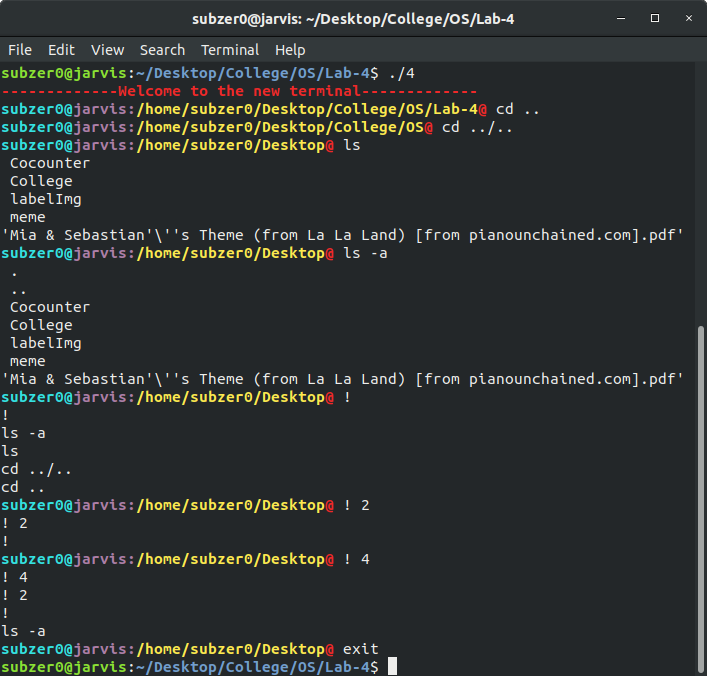
\includegraphics[width=\textwidth]{output/4.png}
\end{figure}
\bigskip
\bigskip
\bigskip

\bigskip



\section*{Question 5: Develop a multiprocessing version of Histogram generator to count the occurrence of various characters in a given text.}
\bigskip

\textbf{\Large Code:}
\smallskip
\par\noindent\rule{\textwidth}{0.4pt}
\lstinputlisting[language=c]{src/5.c}
\par\noindent\rule{\textwidth}{0.4pt}

\bigskip
\noindent
\textbf{\Large Explanation: } \\
% \bigskip
  \\This code generates a histogram of the letters used in a given string. This
  code uses a multiprocessing approach. For every unique letter, a new process 
  is created to count its occurrence. Once each process traverses the string, 
  each of them prints the character they were responsible for and their respective
  count.
  \\Shared memory was used to maintain a visit array (basically keeps track of 
  all the unique characters) to make sure multiple processes don't count the same 
  character.

\bigskip
\noindent
\textbf{\Large Output:}

\begin{figure}[h]
	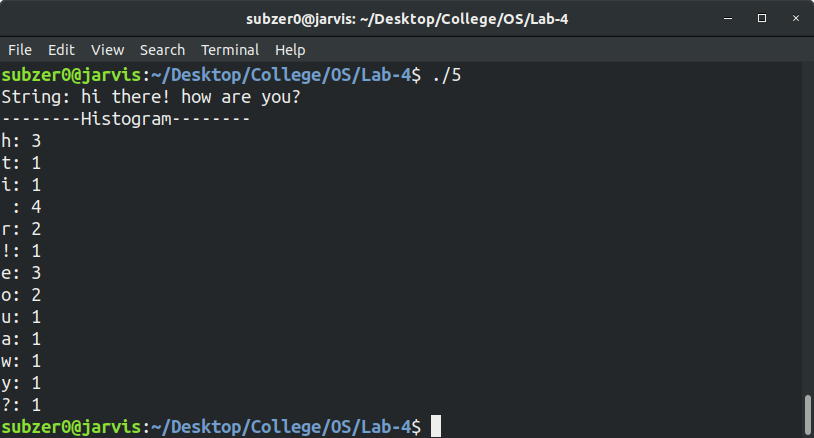
\includegraphics[width=\textwidth]{output/5.png}
\end{figure}
\bigskip
\bigskip
\bigskip

\bigskip


\section*{Question 6: Develop a multiprocessing version of matrix multiplication. Say for a result 3*3 matrix the most efficient form of parallelization can be 9 processes, each of which computes the net resultant value of a row (matrix1) multiplied by column (matrix2). For programmers convenience you can start with 4 processes, but as I said each result value can be computed parallel independent of the other processes in execution.}
\bigskip

\textbf{\Large Code:}
\smallskip
\par\noindent\rule{\textwidth}{0.4pt}
\lstinputlisting[language=c]{src/6.c}
\par\noindent\rule{\textwidth}{0.4pt}

\bigskip
\noindent
\textbf{\Large Explanation: } \\

Appropriately placed fork calls with shared memory in the usual matrix multiplication algorithm 
ensures that a multiprocessing version of matrix multiplication can be achieved.

\bigskip
\noindent
\textbf{\Large Output:}

\begin{figure}[h]
	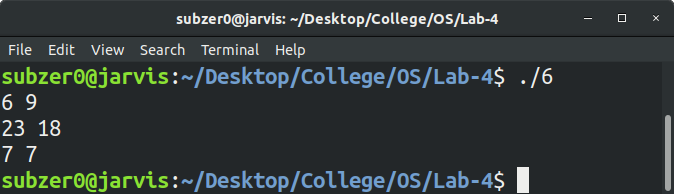
\includegraphics[width=\textwidth]{output/6.png}
\end{figure}
\bigskip
\bigskip
\bigskip

\bigskip

\end{document}